\chapter{Memory as an engine}

\label{ch:memory-engine}

The administrator's chapter describes memory as documents and layers. This one describes the
machinery that makes them findable: the crate, the three lanes and their contracts, the fusion,
the decay, the quantisation, and the consolidation algorithm with its caps. Every constant quoted
here is read from the code, and the tests named are the ones that would fail if it changed.

\section{One crate, ten responsibilities}

\texttt{pii-memory} is the whole ranking surface. Nothing else in the workspace computes a memory
score, and nothing in it opens a store directly --- it takes an \texttt{Arc<MemStore>} and a
\texttt{Ctx}.

\begin{longtable}{@{}p{0.22\textwidth}p{0.54\textwidth}p{0.18\textwidth}@{}}
  \toprule
  \textbf{Module} & \textbf{Responsibility} & \textbf{Touches models?} \\
  \midrule
  \endhead
  \texttt{doc.rs} & \texttt{Layer} (L1--L3), \texttt{DocKind} (atom, scene, persona, skill), the \texttt{Doc} record & no \\
  \texttt{tokenize.rs} & the one tokeniser, so BM25 and concepts agree on what a word is & no \\
  \texttt{bm25.rs} & lexical lane: term overlap, corpus statistics & no \\
  \texttt{embed.rs} & embeddings, behind an optional \texttt{Embedder} & yes, if configured \\
  \texttt{vector.rs} & vector lane over int8-quantised vectors & no (uses stored vectors) \\
  \texttt{quant.rs} & \texttt{quantise}, \texttt{dot\_i8}, \texttt{cosine\_q} & no \\
  \texttt{graph\_lane.rs} & concept co-occurrence expansion, label propagation & \textbf{no, zero model calls} \\
  \texttt{rrf.rs} & reciprocal-rank fusion and \texttt{decayed} & no \\
  \texttt{decay.rs} & the $\lambda$ constants, one per kind & no \\
  \texttt{consolidate.rs} & candidate generation, merge rules, caps, archival recommendation & no \\
  \bottomrule
\end{longtable}

The right-hand column is the load-bearing one. Exactly one module can call a model, and it is
optional: an installation with no embedder runs two lanes and says so. That is a deliberate
property of the design --- memory retrieval is not allowed to become a model dependency.

\section{The search, in order}

\begin{center}
\resizebox{\linewidth}{!}{
\begin{tikzpicture}[node distance=8mm and 10mm]
  \node[b] (tok) {tokenise\\\scriptsize tokenize.rs};
  \node[b, right=of tok, yshift=13mm] (bm) {BM25\\\scriptsize ranked ids};
  \node[b, right=of tok] (vec) {vector\\\scriptsize if embedder};
  \node[b, right=of tok, yshift=-13mm] (gr) {graph\\\scriptsize if concepts match};
  \node[b, right=of vec, yshift=13mm] (rrf) {RRF k=60};
  \node[b, right=of rrf, yshift=13mm] (dec) {decay per kind};
  \node[b, below=of dec] (res) {MemorySearchResult\\\scriptsize hits · lanes · degraded};
  \draw[f] (tok) -- (bm); \draw[f] (tok) -- (vec); \draw[f] (tok) -- (gr);
  \draw[f] (bm) -- (rrf); \draw[f] (vec) -- (rrf); \draw[f] (gr) -- (rrf);
  \draw[f] (rrf) -- (dec); \draw[f] (dec) -- (res);
\end{tikzpicture}}
\captionof{figure}{The result carries its own evidence: which lanes ran, and whether the vector lane was skipped. A caller never has to guess why the answer is what it is.}
\end{center}

The result type is the contract:

\begin{lstlisting}[language=bash]
MemorySearchResult { hits, lanes: Vec<String>, degraded: bool }
    lanes     the lanes that RAN (not the lanes that HIT)
    degraded  the vector lane was skipped: embedder error, or dims() == 0
\end{lstlisting}

\texttt{lanes} being ``ran'' rather than ``hit'' is the single most misread field in the crate, and
it produced real confusion in operator use before it was written down. A lane that ran and found
nothing looks identical to a lane that ran and found everything, from the caller's side, unless the
caller also looks at the hits.

\section{Fusion: why ranks, and not scores}

The three lanes produce incomparable numbers. BM25 is unbounded and corpus-dependent; cosine
similarity is bounded in $[-1,1]$; the graph lane counts hops. Averaging them would let whichever
lane has the largest numeric range dominate every result.

Reciprocal-rank fusion avoids the problem by discarding magnitude and keeping order:

\begin{center}
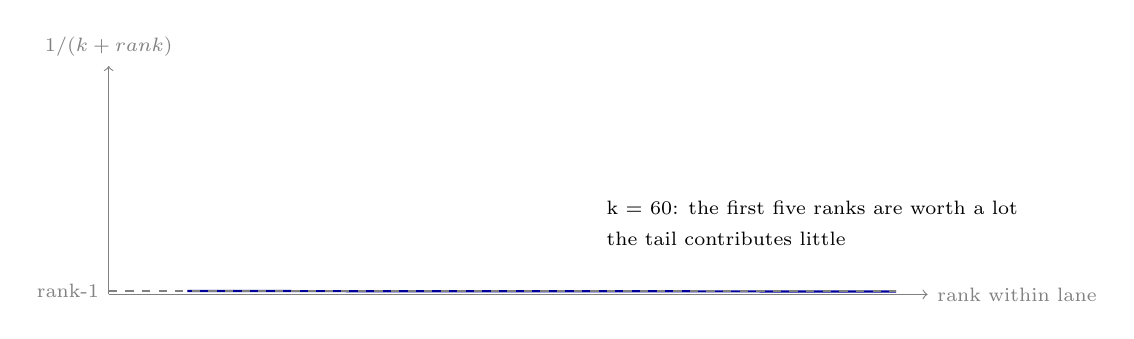
\begin{tikzpicture}[x=1cm,y=1cm]
  \draw[->, gray] (0,0) -- (10.4,0) node[right, font=\scriptsize] {rank within lane};
  \draw[->, gray] (0,0) -- (0,2.9) node[above, font=\scriptsize] {$1/(k+\text{rank})$};
  \draw[thick, blue!60!black] plot[domain=1:10, samples=60] (\x, {2.6/(60+\x)});
  \node[font=\scriptsize, right] at (6.2,1.1) {k = 60: the first five ranks are worth a lot};
  \node[font=\scriptsize, right] at (6.2,0.7) {the tail contributes little};
  \draw[dashed, gray] (0, {2.6/61}) -- (10, {2.6/61});
  \node[font=\scriptsize, gray, left] at (0,{2.6/61}) {rank-1};
\end{tikzpicture}
\captionof{figure}{$k=60$ flattens the top of the curve: rank 1 and rank 3 are close, which is what lets two lanes agree and beat one confident lane.}
\end{center}

With $k=60$ fixed in \texttt{rrf.rs::RRF\_K}, the fusion is deterministic and testable: the same
three ranked lists always produce the same fused list, so a test can assert an exact ordering
rather than a property.

\section{Decay, and why it is per kind}

Decay multiplies the fused score by $e^{-\lambda\,\text{age\_days}}$, with $\lambda$ taken from the
kind:

\begin{longtable}{@{}p{0.20\textwidth}p{0.16\textwidth}p{0.20\textwidth}p{0.36\textwidth}@{}}
  \toprule
  \textbf{Kind} & \textbf{$\lambda$} & \textbf{Half-life} & \textbf{Why} \\
  \midrule
  \endhead
  atom & 0.02 & 34.7 days & a single observation ages fast; the world moves \\
  scene & 0.005 & 138.6 days & a distillation of atoms outlives any one of them \\
  skill & 0.001 & 693.1 days & a procedure stays true far longer than the facts behind it \\
  persona & 0.0 & never & identity is not a claim about the world \\
  \bottomrule
\end{longtable}

The function is pure --- \texttt{decayed(score, kind, age\_days)} --- and the age comes from
\texttt{Ctx::now\_ms()}, which is what makes decay testable without waiting: a test sets the clock,
not the calendar. That detail matters because the first version of these tests used the wall clock
and became the subject of a separate row.

\section{Quantisation: what the vector lane actually stores}

Vectors are stored as \texttt{i8}, not \texttt{f32}, with a per-vector scale factor:

\begin{lstlisting}[language=bash]
quantise(v: &[f32]) -> (Vec<i8>, f32)   # values + the scale needed to undo them
dot_i8(a, b) -> i32                      # integer dot product
cosine_q(a, sa, b, sb) -> f32            # cosine from quantised pairs and their scales
\end{lstlisting}

The consequence for an operator is storage: a 768-dimension vector costs 768 bytes plus a scale
rather than 3\,072. The consequence for a developer is that the vector lane's similarity is an
approximation, and a test that asserts exact float equality against an unquantised baseline is
wrong by construction.

\section{Consolidation, algorithmically}

Candidate generation walks documents and proposes merges; the rules decide whether a proposal
becomes a scene. The constants are in \texttt{consolidate.rs}:

\begin{longtable}{@{}p{0.34\textwidth}p{0.16\textwidth}p{0.42\textwidth}@{}}
  \toprule
  \textbf{Constant} & \textbf{Value} & \textbf{Effect} \\
  \midrule
  \endhead
  \texttt{MIN\_SHARED\_CONCEPTS} & 2 & one shared word cannot start a merge \\
  \texttt{MIN\_CONCEPT\_JACCARD} & 0.15 & guards against merging documents that merely share a topic \\
  \texttt{NEGATION\_WINDOW} & 8 tokens & a negation near a shared concept vetoes the merge \\
  \texttt{MAX\_CANDIDATES} & 200 & generation stops at 200; the report says \texttt{candidates\_capped} \\
  \texttt{same\_layer\_only} & true & merges never cross layers \\
  \texttt{archive\_after\_days} & configured & last-use age at which a document is archived \\
  \bottomrule
\end{longtable}

The report is as important as the merge: \texttt{candidates\_evaluated}, \texttt{candidates\_capped},
\texttt{merged}. A capped run is not a failed run; it is a run that stopped early and said so, and
the correct response is to run it again rather than to raise the cap.

\section{The store underneath}

Memory does not get its own writer. Documents and edges live in the same store as everything else,
written through the same single write path, which is why a second daemon cannot corrupt memory
without first having corrupted the store (chapter~6). The tables an operator will meet are the
document table and the edge table; \texttt{mem\_edge} is what the graph lane traverses, and an
empty edge table is precisely why that lane contributes nothing.

\begin{center}
\resizebox{\linewidth}{!}{
\begin{tikzpicture}[node distance=9mm and 12mm]
  \node[b] (put) {memory put\\\scriptsize daemon only};
  \node[b, right=of put] (doc) {document\\\scriptsize id = blake3(text)};
  \node[s, right=of doc] (store) {store\\\scriptsize one writer};
  \node[b, below=of doc] (edge) {edges\\\scriptsize concept co-occurrence};
  \node[b, below=of store] (lane) {graph lane\\\scriptsize reads edges only};
  \draw[f] (put) -- (doc); \draw[f] (doc) -- (store);
  \draw[sf] (doc) -- (edge); \draw[f] (edge) -- (lane);
  \draw[bk] (lane.west) to[bend right=14] node[p,below]{nothing to traverse} (doc.south);
\end{tikzpicture}}
\captionof{figure}{Writes create both the document and its edges; the lane reads only edges. A store written without concepts has documents, no edges, and one silent lane.}
\end{center}

\section{What would break, and which test notices}

\begin{longtable}{@{}p{0.32\textwidth}p{0.36\textwidth}p{0.26\textwidth}@{}}
  \toprule
  \textbf{Change} & \textbf{Visible symptom} & \textbf{Test that objects} \\
  \midrule
  \endhead
  $\lambda$ raised for atoms & old facts vanish from the top of results & decay table tests \\
  $k$ changed in RRF & orderings shift; two lanes stop agreeing & fusion ordering tests \\
  quantisation removed & storage grows; vector similarity changes & quant round-trip tests \\
  concept recording dropped & graph lane stops contributing, still reports running & \texttt{lanes.rs::graph\_lane\_recalls\_doc\_via\_shared\_concept} \\
  embedder made mandatory & installations without a model stop answering & degraded-lane tests \\
  negation window ignored & scenes assert contradictory facts & consolidation veto tests \\
  cap removed & consolidation becomes unbounded work & cap-report tests \\
  \bottomrule
\end{longtable}

The second row of that table is the one to keep in mind when reading memory code: every constant
here is a behaviour, and the tests are written against orderings and counts rather than against
scores, so a change to any of them fails a test rather than silently changing what pii remembers
first.
